% XeLaTeX

\documentclass{article}
\usepackage{ctex}
\usepackage{xypic}
\usepackage{amsfonts,amssymb}
\usepackage{multirow}
\usepackage{geometry}
\usepackage{graphicx}
\usepackage{listings}
\usepackage{lipsum}
\usepackage{courier}
\usepackage{fancyvrb}
\usepackage{etoolbox}


\linespread{1.2}
\geometry{left=3cm,right=2.5cm,top=2.5cm,bottom=2.5cm}

\makeatletter
\patchcmd{\FV@SetupFont}
  {\FV@BaseLineStretch}
  {\fontencoding{T1}\FV@BaseLineStretch}
  {}{}
\makeatother

\lstset{basicstyle=\small\fontencoding{T1}\ttfamily,breaklines=true}
\lstset{numbers=left,frame=shadowbox,tabsize=4}
%\lstset{extendedchars=false}
\begin{document}

\title{数据库系统实验1 \ 实验报告}
\author {数据科学与计算机学院 \ 计算机科学与技术 2016 级 \\ 王凯祺 \ 16337233}
\maketitle

\section{实验1.1 数据库定义实验}

本实验建立大学数据库模式。大学数据库模式由教室(classroom)、院系(department)、课程科目(course)、导师(instructor)、课程(section)、任教(teaches)、学生(student)、选课(takes)、推荐(advisor)、时间段(time\_slot)、课程约束(prereq)共 11 个表组成。

\begin{figure}[!hbp]
\centering
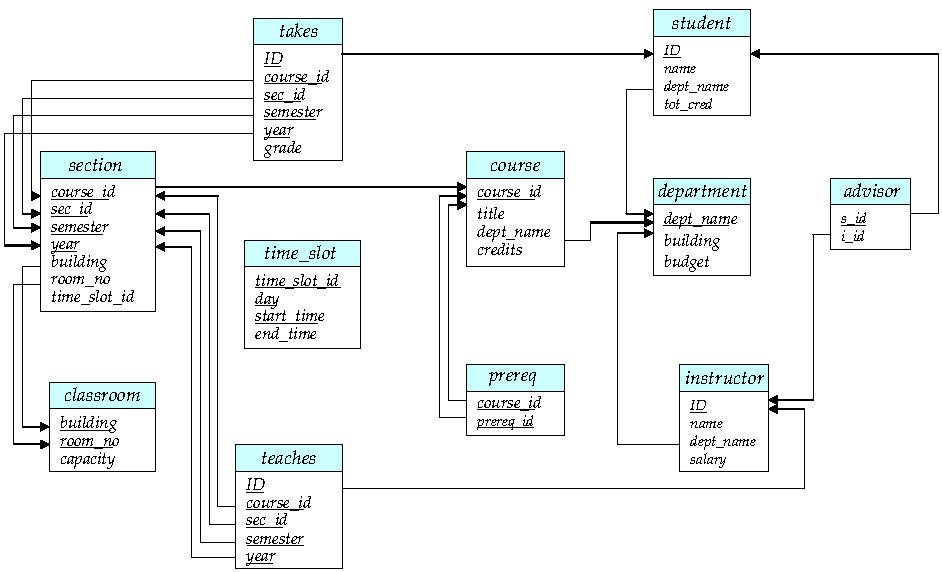
\includegraphics[scale=1.0]{a.jpg}
\end{figure}

我采用 Mysql 8.0 来做本次实验。

\subsection{定义数据库}

创建一个名为 lab 的数据库。

\begin{lstlisting}[language=sql]
create database lab;
\end{lstlisting}

这样创建出来的数据库模式是默认的,大小写不敏感。

\subsection{定义基本表}

在 lab 数据库中创建 11 个表。

\begin{lstlisting}[language=sql]
create table classroom
	(building		varchar(15),
	 room_number		varchar(7),
	 capacity		numeric(4,0),
	 primary key (building, room_number)
	);
create table department
	(dept_name		varchar(20), 
	 building		varchar(15), 
	 budget		        numeric(12,2) check (budget > 0),
	 primary key (dept_name)
	);
create table course
	(course_id		varchar(8), 
	 title			varchar(50), 
	 dept_name		varchar(20),
	 credits		numeric(2,0) check (credits > 0),
	 primary key (course_id),
	 foreign key (dept_name) references department(dept_name)
		on delete set null
	);
create table instructor
	(ID			varchar(5), 
	 name			varchar(20) not null, 
	 dept_name		varchar(20), 
	 salary			numeric(8,2) check (salary > 29000),
	 primary key (ID),
	 foreign key (dept_name) references department(dept_name)
		on delete set null
	);
create table section
	(course_id		varchar(8), 
         sec_id			varchar(8),
	 semester		varchar(6)
		check (semester in ('Fall', 'Winter', 'Spring', 'Summer')), 
	 year			numeric(4,0) check (year > 1701 and year < 2100), 
	 building		varchar(15),
	 room_number		varchar(7),
	 time_slot_id		varchar(4),
	 primary key (course_id, sec_id, semester, year),
	 foreign key (course_id) references course(course_id)
		on delete cascade,
	 foreign key (building, room_number) references classroom(building, room_number)
		on delete set null
	);
create table teaches
	(ID			varchar(5), 
	 course_id		varchar(8),
	 sec_id			varchar(8), 
	 semester		varchar(6),
	 year			numeric(4,0),
	 primary key (ID, course_id, sec_id, semester, year),
	 foreign key (course_id,sec_id, semester, year) references section(course_id,sec_id, semester, year)
		on delete cascade,
	 foreign key (ID) references instructor(ID)
		on delete cascade
	);
create table student
	(ID			varchar(5), 
	 name			varchar(20) not null, 
	 dept_name		varchar(20), 
	 tot_cred		numeric(3,0) check (tot_cred >= 0),
	 primary key (ID),
	 foreign key (dept_name) references department(dept_name)
		on delete set null
	);
create table takes
	(ID			varchar(5), 
	 course_id		varchar(8),
	 sec_id			varchar(8), 
	 semester		varchar(6),
	 year			numeric(4,0),
	 grade		        varchar(2),
	 primary key (ID, course_id, sec_id, semester, year),
	 foreign key (course_id,sec_id, semester, year) references section(course_id,sec_id, semester, year)
		on delete cascade,
	 foreign key (ID) references student(ID)
		on delete cascade
	);
create table advisor
	(s_ID			varchar(5),
	 i_ID			varchar(5),
	 primary key (s_ID),
	 foreign key (i_ID) references instructor (ID)
		on delete set null,
	 foreign key (s_ID) references student (ID)
		on delete cascade
	);
create table time_slot
	(time_slot_id		varchar(4),
	 day			varchar(1),
	 start_hr		numeric(2) check (start_hr >= 0 and start_hr < 24),
	 start_min		numeric(2) check (start_min >= 0 and start_min < 60),
	 end_hr			numeric(2) check (end_hr >= 0 and end_hr < 24),
	 end_min		numeric(2) check (end_min >= 0 and end_min < 60),
	 primary key (time_slot_id, day, start_hr, start_min)
	);
create table prereq
	(course_id		varchar(8), 
	 prereq_id		varchar(8),
	 primary key (course_id, prereq_id),
	 foreign key (course_id) references course(course_id)
		on delete cascade,
	 foreign key (prereq_id) references course(course_id)
	)
\end{lstlisting}

\subsection{实验数据准备}

实验使用的 DDL 和数据均从 http://www.db-book.com 下载。

\subsection{思考题}

(1) SQL 语法规定,双引号括定的符号串为对象名称,单引号括定的符号串为常量字符串,那么什么情况下需要用双引号来界定对象名呢?

在 Mysql 中,当对象名称恰为 SQL 保留字时,需用反引号括定,避免歧义。

(2) 数据库对象的完整引用是“服务器名.数据库名.模式名.对象名”,但通常可以省略服务器名和数据库名,甚至模式名,直接用对象名访问对象即可。

使用 mysql 进行数据库连接时,已经提供了服务器名,故可以默认省略服务器名。

建立连接后,使用 use $database$; 选定默认数据库。

省略模式名通常在 from 后面只有一个表,或者有多个表但对象名在这多个表中只出现一次。

\subsection{实验总结}

通过实验,我能读懂表头信息,相当于 excel 表的第一行。每一列指定一个数据类型用于存放数据,这类似于 C++ 。 primary key 是主键,它默认是索引,可提高查询效率; foreign key 是外键,用于连接到别的表。

\section{实验1.2 数据基本查询实验}

\subsection{单表查询(实现投影操作)}

查询学生 ID 、姓名。

\begin{lstlisting}[language=sql]
select ID, name from student limit 10;
\end{lstlisting}

结果为:

\begin{lstlisting}
+-------+-----------+
| ID    | name      |
+-------+-----------+
| 1000  | Manber    |
| 10033 | Zelty     |
| 10076 | Duan      |
| 1018  | Colin     |
| 10204 | Mediratta |
| 10267 | Rzecz     |
| 10269 | Hilberg   |
| 10454 | Ugarte    |
| 10481 | Grosch    |
| 10527 | Kieras    |
+-------+-----------+
10 rows in set (0.01 sec)
\end{lstlisting}

\subsection{单表查询(实现选择操作)}

查询 2009 年春季学期开设的课程 ID 。

\begin{lstlisting}[language=sql]
select course_id from section where semester = 'Spring' and year = '2009';
\end{lstlisting}

\begin{lstlisting}
+-----------+
| course_id |
+-----------+
| 604       |
| 972       |
+-----------+
2 rows in set (0.01 sec)
\end{lstlisting}

\subsection{不带分组过滤条件的分组统计查询}

统计每个学生选的课程数。

\begin{lstlisting}[language=sql]
select S.ID, S.name, count(T.course_id) 
from student as S, takes as T 
where S.ID = T.ID 
group by S.ID limit 10;
\end{lstlisting}

\begin{lstlisting}
+-------+-----------+--------------------+
| ID    | name      | count(T.course_id) |
+-------+-----------+--------------------+
| 1000  | Manber    |                 13 |
| 10033 | Zelty     |                 22 |
| 10076 | Duan      |                 14 |
| 1018  | Colin     |                 22 |
| 10204 | Mediratta |                 12 |
| 10267 | Rzecz     |                 11 |
| 10269 | Hilberg   |                 10 |
| 10454 | Ugarte    |                 18 |
| 10481 | Grosch    |                 17 |
| 10527 | Kieras    |                 21 |
+-------+-----------+--------------------+
10 rows in set (0.01 sec)
\end{lstlisting}

\subsection{带分组过滤条件的分组统计查询}

查询选课数超过 25 的学生 ID 和姓名。

\begin{lstlisting}[language=sql]
select S.ID, max(S.name)
from student as S, takes as T
where S.ID = T.ID group by S.ID
having count(T.course_id) > 25;
\end{lstlisting}

\begin{lstlisting}
+-------+-------------+
| ID    | max(S.name) |
+-------+-------------+
| 12078 | Knutson     |
| 44551 | Nguyen      |
| 72669 | Schmitz     |
| 79170 | Lingamp     |
| 90448 | Godfrey     |
+-------+-------------+
5 rows in set (0.05 sec)
\end{lstlisting}

\subsection{单表自身连接查询}

查询比其中一个计算机系学生获得的学分高的所有学生 ID 和姓名。

\begin{lstlisting}[language=sql]
select distinct S.ID, S.name
from student as S, student as T
where T.dept_name = 'Comp. Sci.' and S.tot_cred > T.tot_cred limit 10;
\end{lstlisting}

\begin{lstlisting}
+-------+-----------+
| ID    | name      |
+-------+-----------+
| 1000  | Manber    |
| 10033 | Zelty     |
| 10076 | Duan      |
| 1018  | Colin     |
| 10204 | Mediratta |
| 10267 | Rzecz     |
| 10269 | Hilberg   |
| 10454 | Ugarte    |
| 10481 | Grosch    |
| 10527 | Kieras    |
+-------+-----------+
10 rows in set (0.01 sec)
\end{lstlisting}

\subsection{三表连接查询}

查询所有课程的课程名和教授。

\begin{lstlisting}[language=sql]
select distinct C.title, I.name
from instructor as I, teaches as T, course as C
where I.ID = T.ID and T.course_id = C.course_id limit 10;
\end{lstlisting}

\begin{lstlisting}
+--------------------------+------------+
| title                    | name       |
+--------------------------+------------+
| Image Processing         | Romero     |
| Manufacturing            | Mingoz     |
| Elastic Structures       | Bietzk     |
| Elastic Structures       | Dale       |
| Marine Mammals           | Gustafsson |
| Drama                    | Liley      |
| The Music of the Ramones | Lembr      |
| The Music of the Ramones | Ullman     |
| Surfing                  | Dale       |
| The Music of the Ramones | Voronina   |
+--------------------------+------------+
10 rows in set (0.07 sec)
\end{lstlisting}

\subsection{实验总结}

不在 group by 子句出现的属性,可以出现在 select 子句中,但必须用聚集函数(avg, min, max, sum, count)。

在分组统计查询中, where 条件针对的是单个元组,而 having 条件针对的是 group by 子句构成的分组。

如:查询教师平均工资超过 42000 美元的系可以这样写

\begin{lstlisting}[language=sql]
select dept_name, avg(salary) as avg_salary
from instructor
group by dept_name
having avg(salary) > 42000;
\end{lstlisting}

\section{实验1.3 数据高级查询实验}

\subsection{IN 嵌套查询}

查询选了 Kean 老师的课的所有学生(学号、姓名)。

\begin{lstlisting}[language=sql]
select `ID`, `name`
from `student`
where `ID` in
	(select `takes`.`ID`
	from `takes`, `teaches`, `instructor`
    where `takes`.`course_id` = `teaches`.`course_id` and
		`takes`.`sec_id` = `teaches`.`sec_id` and
        `takes`.`year` = `teaches`.`year` and
        `takes`.`semester` = `teaches`.`semester` and
		`teaches`.`ID` = `instructor`.`ID` and
        `instructor`.`name` = 'Kean');
limit 10;
\end{lstlisting}

结果如下:

\begin{lstlisting}
+-------+------------+
| ID    | name       |
+-------+------------+
| 10267 | Rzecz      |
| 107   | Shabuno    |
| 10736 | Veselovsky |
| 10834 | More       |
| 11152 | Al-Tahat   |
| 11419 | Geronimo   |
| 11453 | Yamashita  |
| 11855 | Mendelzon  |
| 12563 | Stone      |
| 13028 | Okano      |
+-------+------------+
10 rows in set (0.02 sec)
\end{lstlisting}

\subsection{单层 exists 嵌套查询}

查询没有选 Kean 老师的课的所有学生(学号、姓名)。

\begin{lstlisting}[language=sql]
select `ID`, `name`
from `student`
where not exists
	(select `takes`.`ID`
	from `takes`, `teaches`, `instructor`
    where `student`.`ID` = `takes`.`ID` and
		`takes`.`course_id` = `teaches`.`course_id` and
		`takes`.`sec_id` = `teaches`.`sec_id` and
        `takes`.`year` = `teaches`.`year` and
        `takes`.`semester` = `teaches`.`semester` and
		`teaches`.`ID` = `instructor`.`ID` and
        `instructor`.`name` = 'Kean');
\end{lstlisting}

结果如下:

\begin{lstlisting}
+-------+------------+
| ID    | name       |
+-------+------------+
| 5144  | Abdellatif |
| 45002 | Abraham    |
| 20244 | Abu-B      |
| 83622 | Achilles   |
| 13511 | Adam       |
| 20084 | Adda       |
| 46655 | Advani     |
| 58326 | Afim       |
| 18709 | Agar       |
| 49205 | Agraz      |
+-------+------------+
10 rows in set (0.20 sec)
\end{lstlisting}

\subsection{双层 exists 嵌套查询}

查询至少选了 Manber 选过的所有课程的学生(学号、姓名)。

\begin{lstlisting}[language=sql]
select `ID`, `name`
from `student` as S2
where not exists
	(select 1
    from `takes` as T1, `student` as S1
    where T1.`ID` = S1.`ID` and
		S1.`name` = 'Manber' and
        not exists (
			select 1
            from `takes` as T2
            where T2.`course_id` = T1.`course_id` and
				T2.`ID` = S2.`ID`
        )
	);
\end{lstlisting}

结果如下:

\begin{lstlisting}
+------+--------+
| ID   | name   |
+------+--------+
| 1000 | Manber |
+------+--------+
1 row in set (0.05 sec)
\end{lstlisting}

\subsection{from 子句中的嵌套查询}

查询选课数超过 20 门的学生。

\begin{lstlisting}[language=sql]
select S.`ID`, S.`name`, T.cnt
from `student` as S,
	(select `ID`, count(`course_id`) as cnt
    from `takes`
    group by `ID`) as T
where S.ID = T.ID and T.cnt > 20
limit 10;
\end{lstlisting}

结果如下:

\begin{lstlisting}
+-------+---------+-----+
| ID    | name    | cnt |
+-------+---------+-----+
| 10033 | Zelty   |  22 |
| 1018  | Colin   |  22 |
| 10527 | Kieras  |  21 |
| 107   | Shabuno |  25 |
| 10834 | More    |  22 |
| 12078 | Knutson |  27 |
| 1367  | Ignj    |  21 |
| 14432 | Whitley |  22 |
| 14639 | Sagiv   |  21 |
| 14668 | Malinen |  23 |
+-------+---------+-----+
10 rows in set (0.07 sec)
\end{lstlisting}

\subsection{集合查询(交)}

查询 Zelty 和 Colin 都选过的所有课。

mysql 没有 intersect 运算符。好在我们可以使用 inner join 代替它。

\begin{lstlisting}[language=sql]
select tab1.course_id, tab1.sec_id, tab1.semester, tab1.year from 
(select T1.*
from `student` as S1, `takes` as T1
where S1.ID = T1.ID and S1.name = 'Zelty') as tab1
join
(select T2.*
from `student` as S2, `takes` as T2
where S2.ID = T2.ID and S2.name = 'Colin') as tab2
on tab1.`course_id` = tab2.`course_id`;
\end{lstlisting}

结果如下:

\begin{lstlisting}
+-----------+--------+----------+------+
| course_id | sec_id | semester | year |
+-----------+--------+----------+------+
| 338       | 1      | Spring   | 2007 |
| 338       | 2      | Spring   | 2006 |
| 362       | 3      | Spring   | 2008 |
| 457       | 1      | Spring   | 2001 |
| 603       | 1      | Fall     | 2003 |
| 791       | 1      | Spring   | 2006 |
| 972       | 1      | Spring   | 2009 |
+-----------+--------+----------+------+
7 rows in set (0.11 sec)

\end{lstlisting}

\subsection{集合查询(并)}

查询 Zelty 和 Colin 选过的所有课。

\begin{lstlisting}[language=sql]
(select T1.*
from `student` as S1, `takes` as T1
where S1.ID = T1.ID and S1.name = 'Zelty')
union
(select T2.*
from `student` as S2, `takes` as T2
where S2.ID = T2.ID and S2.name = 'Colin')
\end{lstlisting}

结果如下:

\begin{lstlisting}
+-------+-----------+--------+----------+------+-------+
| ID    | course_id | sec_id | semester | year | grade |
+-------+-----------+--------+----------+------+-------+
| 10033 | 242       | 1      | Fall     | 2009 | B     |
| 10033 | 334       | 1      | Fall     | 2009 | C-    |
| 10033 | 338       | 1      | Spring   | 2007 | A     |
| 10033 | 338       | 2      | Spring   | 2006 | C     |
| 10033 | 352       | 1      | Spring   | 2006 | A     |
| 10033 | 362       | 3      | Spring   | 2008 | A-    |
| 10033 | 408       | 1      | Spring   | 2007 | C-    |
| 10033 | 408       | 2      | Spring   | 2003 | B+    |
| 10033 | 443       | 2      | Spring   | 2002 | C-    |
| 10033 | 445       | 1      | Spring   | 2001 | C     |
| 10033 | 457       | 1      | Spring   | 2001 | C-    |
| 10033 | 486       | 1      | Fall     | 2009 | C     |
| 10033 | 493       | 1      | Spring   | 2010 | C-    |
| 10033 | 603       | 1      | Fall     | 2003 | B     |
| 10033 | 604       | 1      | Spring   | 2009 | A-    |
| 10033 | 629       | 1      | Spring   | 2003 | B-    |
| 10033 | 679       | 1      | Spring   | 2010 | A+    |
| 10033 | 692       | 1      | Spring   | 2010 | A     |
| 10033 | 702       | 1      | Spring   | 2001 | A     |
| 10033 | 791       | 1      | Spring   | 2006 | C     |
| 10033 | 960       | 1      | Fall     | 2009 | C+    |
| 10033 | 972       | 1      | Spring   | 2009 | C+    |
| 1018  | 105       | 1      | Fall     | 2009 | A     |
| 1018  | 158       | 1      | Fall     | 2008 | A-    |
| 1018  | 192       | 1      | Fall     | 2002 | B     |
| 1018  | 200       | 2      | Fall     | 2002 | B-    |
| 1018  | 239       | 1      | Fall     | 2006 | B-    |
| 1018  | 274       | 1      | Fall     | 2002 | A+    |
| 1018  | 304       | 1      | Fall     | 2009 | B     |
| 1018  | 319       | 1      | Spring   | 2003 | C     |
| 1018  | 338       | 1      | Spring   | 2007 | A     |
| 1018  | 349       | 1      | Spring   | 2008 | A-    |
| 1018  | 362       | 3      | Spring   | 2008 | B     |
| 1018  | 401       | 1      | Fall     | 2003 | C     |
| 1018  | 421       | 1      | Fall     | 2004 | C-    |
| 1018  | 457       | 1      | Spring   | 2001 | B+    |
| 1018  | 468       | 1      | Fall     | 2005 | B     |
| 1018  | 476       | 1      | Fall     | 2010 | B+    |
| 1018  | 482       | 1      | Fall     | 2005 | A+    |
| 1018  | 581       | 1      | Spring   | 2005 | B     |
| 1018  | 599       | 1      | Spring   | 2003 | A+    |
| 1018  | 603       | 1      | Fall     | 2003 | C+    |
| 1018  | 791       | 1      | Spring   | 2006 | B     |
| 1018  | 972       | 1      | Spring   | 2009 | C-    |
+-------+-----------+--------+----------+------+-------+
44 rows in set (0.12 sec)
\end{lstlisting}

\subsection{集合查询(差)}

查询 Zelty 选过,但 Colin 没选过的所有课。

mysql 没有 except 运算符,好在我们可以使用两种方法代替 except :

\begin{itemize}
\item select form table1 where not in (select from table2)
\item 运用在B不在A中的项用Left Join 会填入NULL这一性质
\end{itemize}

\begin{lstlisting}[language=sql]
select T1.*
from `student` as S1, `takes` as T1
where S1.ID = T1.ID and 
	S1.name = 'Zelty' and
    T1.`course_id` not in
	(select T2.`course_id`
	from `student` as S2, `takes` as T2
	where S2.ID = T2.ID and S2.name = 'Colin')
\end{lstlisting}

\begin{lstlisting}[language=sql]
select tab1.* from (
	(select T1.*
	from `student` as S1, `takes` as T1
	where S1.ID = T1.ID and 
		S1.name = 'Zelty') as tab1
	left join
	(select T2.*
	from `student` as S2, `takes` as T2
	where S2.ID = T2.ID and
		S2.name = 'Colin') as tab2
	on tab1.`course_id` = tab2.`course_id`)
where tab2.ID is null;
\end{lstlisting}


用第一种方法实现,结果如下:

\begin{lstlisting}
+-------+-----------+--------+----------+------+-------+
| ID    | course_id | sec_id | semester | year | grade |
+-------+-----------+--------+----------+------+-------+
| 10033 | 242       | 1      | Fall     | 2009 | B     |
| 10033 | 334       | 1      | Fall     | 2009 | C-    |
| 10033 | 352       | 1      | Spring   | 2006 | A     |
| 10033 | 408       | 1      | Spring   | 2007 | C-    |
| 10033 | 408       | 2      | Spring   | 2003 | B+    |
| 10033 | 443       | 2      | Spring   | 2002 | C-    |
| 10033 | 445       | 1      | Spring   | 2001 | C     |
| 10033 | 486       | 1      | Fall     | 2009 | C     |
| 10033 | 493       | 1      | Spring   | 2010 | C-    |
| 10033 | 604       | 1      | Spring   | 2009 | A-    |
| 10033 | 629       | 1      | Spring   | 2003 | B-    |
| 10033 | 679       | 1      | Spring   | 2010 | A+    |
| 10033 | 692       | 1      | Spring   | 2010 | A     |
| 10033 | 702       | 1      | Spring   | 2001 | A     |
| 10033 | 960       | 1      | Fall     | 2009 | C+    |
+-------+-----------+--------+----------+------+-------+
15 rows in set (0.02 sec)

\end{lstlisting}


用第二种方法实现,结果如下:

\begin{lstlisting}
+-------+-----------+--------+----------+------+-------+
| ID    | course_id | sec_id | semester | year | grade |
+-------+-----------+--------+----------+------+-------+
| 10033 | 242       | 1      | Fall     | 2009 | B     |
| 10033 | 334       | 1      | Fall     | 2009 | C-    |
| 10033 | 352       | 1      | Spring   | 2006 | A     |
| 10033 | 408       | 1      | Spring   | 2007 | C-    |
| 10033 | 408       | 2      | Spring   | 2003 | B+    |
| 10033 | 443       | 2      | Spring   | 2002 | C-    |
| 10033 | 445       | 1      | Spring   | 2001 | C     |
| 10033 | 486       | 1      | Fall     | 2009 | C     |
| 10033 | 493       | 1      | Spring   | 2010 | C-    |
| 10033 | 604       | 1      | Spring   | 2009 | A-    |
| 10033 | 629       | 1      | Spring   | 2003 | B-    |
| 10033 | 679       | 1      | Spring   | 2010 | A+    |
| 10033 | 692       | 1      | Spring   | 2010 | A     |
| 10033 | 702       | 1      | Spring   | 2001 | A     |
| 10033 | 960       | 1      | Fall     | 2009 | C+    |
+-------+-----------+--------+----------+------+-------+
15 rows in set (0.01 sec)

\end{lstlisting}

\subsection{思考题}

(1) 试分析什么类型的查询可以用连接查询实现,什么类型的查询只能用嵌套查询实现?

形如

\begin{lstlisting}[language=sql]
select * from table1,table2 where table1.xxx=table2.xxx
\end{lstlisting}

的查询可用连接查询实现。

(2) 试分析不相关子查询和相关子查询的区别。

1. 非相关子查询是独立于外部查询的子查询,子查询总共执行一次,执行完毕后将值传递给外部查询。 

2. 相关子查询的执行依赖于外部查询的数据,外部查询执行一行,子查询就执行一次。 

故非相关子查询比相关子查询效率高。

\subsection{实验总结}

实验中我遇到 mysql 不支持 intersect, except 语法的问题,查询网上的一些资料,知道了“mysql”还有一些方言,用其他的语句来替代 intersect, except 来完成本次实验。

据说 join 比嵌套查询要快,所以我们以后要多多用 join ,少用嵌套查询。

参考资料:https://blog.csdn.net/thor\_w/article/details/68495088

\section{实验1.4 数据更新实验}

\subsection{insert 基本语句(插入全部列的数据)}

插入一条学生记录,要求每列都给一个合理的值。

\begin{lstlisting}[language=sql]
insert into `student`
values (99988, 'XiaoYao', 'Comp. Sci.', 0);
\end{lstlisting}

\subsection{insert 基本语句(插入部分列的数据)}

插入一条学生记录,给出必要的几个字段的值。

\begin{lstlisting}[language=sql]
insert into `student` (`ID`, `name`, `dept_name`, `tot_cred`)
values (99988, 'XiaoYao', 'Comp. Sci.', 0);
\end{lstlisting}

\subsection{批量数据 insert 语句}

创建一个新的学生表,把所有计算机系的学生插入到学生表中。

\begin{lstlisting}[language=sql]
create table student_comp like student; # 复制数据模式,不复制数据
insert into `student_comp`
	select * from `student` where `student`.`dept_name` = 'Comp. Sci.';
\end{lstlisting}

创建一个学生表,记录每个学生选课总数和得到 A 等级以上的课程总数。

\begin{lstlisting}[language=sql]
create table stu2 (
	ID varchar(5) primary key,
    name varchar(20) not null,
    tot_elect int,
    tot_accept int
);
insert into stu2
select S.`ID`, S.`name`, count(distinct T1.`course_id`), count(distinct T2.`course_id`)
from student as S, takes as T1, takes as T2
where S.`ID` = T1.`ID` and 
	S.`ID` = T2.`ID` and 
	T2.`grade` is not null and
    (T2.`grade` = 'A' or T2.`grade` = 'A+') 
group by S.`ID`;
\end{lstlisting}

\subsection{update 语句(修改部分记录的部分列值)}

计算机系的所有老师工资涨 10\% 。

先查询原来的工资:

\begin{lstlisting}[language=sql]
select *
from instructor
where dept_name = 'Comp. Sci.';
\end{lstlisting}

结果如下:

\begin{lstlisting}
+-------+----------+------------+-----------+
| ID    | name     | dept_name  | salary    |
+-------+----------+------------+-----------+
| 3335  | Bourrier | Comp. Sci. |  79189.95 |
| 34175 | Bondi    | Comp. Sci. | 113171.27 |
+-------+----------+------------+-----------+
2 rows in set (0.01 sec)

\end{lstlisting}

\begin{lstlisting}[language=sql]
update instructor
set salary = salary * 1.1
where dept_name = 'Comp. Sci.';
\end{lstlisting}

更新时产生错误:

\begin{lstlisting}[language=sql]
Error Code: 1175. You are using safe update mode and you tried to update a table without a WHERE that uses a KEY column To disable safe mode, toggle the option in Preferences -> SQL Queries and reconnect.
\end{lstlisting}

这是因为 mysql 防止误更新,只需要执行以下命令,再重新执行更新命令即可。

\begin{lstlisting}[language=sql]
set sql_safe_updates = 0;
\end{lstlisting}

执行后产生两个警告:

\begin{lstlisting}[language=sql]
2 row(s) affected, 2 warning(s): 
1265 Data truncated for column 'salary' at row 1 
1265 Data truncated for column 'salary' at row 2 
Rows matched: 2  Changed: 2  Warnings: 2
\end{lstlisting}

这是因为工资的精度是 2 位小数,乘以 1.1 后变为 3 位小数,自动截断。


再查询现在的工资:

\begin{lstlisting}[language=sql]
select *
from instructor
where dept_name = 'Comp. Sci.';
\end{lstlisting}

结果如下:

\begin{lstlisting}
+-------+----------+------------+-----------+
| ID    | name     | dept_name  | salary    |
+-------+----------+------------+-----------+
| 3335  | Bourrier | Comp. Sci. |  87108.95 |
| 34175 | Bondi    | Comp. Sci. | 124488.40 |
+-------+----------+------------+-----------+
2 rows in set (0.02 sec)

\end{lstlisting}

\subsection{delete 基本语句(删除给定条件的所有记录)}

删除工资高于 50000 的教授。

\begin{lstlisting}[language=sql]
create table ins2 select * from instructor; # 先复制一份数据库用于删除
delete from ins2 where salary > 50000;
\end{lstlisting}

删除时产生错误:

\begin{lstlisting}[language=sql]
Error Code: 1175. You are using safe update mode and you tried to update a table without a WHERE that uses a KEY column To disable safe mode, toggle the option in Preferences -> SQL Queries and reconnect.
\end{lstlisting}

这是因为 mysql 防止误删除,只需要执行以下命令,再重新执行删除命令即可。

\begin{lstlisting}[language=sql]
set sql_safe_updates = 0;
\end{lstlisting}

\subsection{实验总结}

实验不难,不过 update, delete 这个防护开关我真的觉得很赞~

现在的 mysql 8.0 版本已经有 sql\_safe\_updates 这个开关啦!而且默认还是开的!有这个开关之后,所有的 update, delete 操作必须要有 where 子句,且必须指定 primary key (主键)才能删除。想当年我用 mysql 5.6 的时候,一手贱忘记加 where ,结果整列都被改掉了……哭瞎QAQ

\section{实验1.5 视图实验}

\subsection{创建视图(省略视图列名)}

创建一个学生选课视图,要求列出学生学号、姓名、科目、学分、上课时间、上课地点等信息。

\begin{lstlisting}[language=sql]
create view stu_takes as
	select S.`ID`, S.`name`, T.`sec_id`, T.`semester`, T.`year`, C.`title`, C.`credits`, SE.`building`, SE.`room_number`, SE.`time_slot_id`
	from `student` as S, `takes` as T, `course` as C natural join `section` as SE
	where S.`ID` = T.`ID` and
		T.`course_id` = C.`course_id`;
\end{lstlisting}

\subsection{创建视图(不能省略视图列名的情况)}

创建一个学生视图,要求列出学生学号、姓名、已修课程数。

\begin{lstlisting}[language=sql]
create view stu2(ID, name, cnt) as
	select S.`ID`, S.`name`, count(T.`course_id`)
    from `student` as S, `takes` as T
    where S.`ID` = T.`ID`
    group by S.`ID`;
\end{lstlisting}

\subsection{创建视图(with check option)}

创建一个选课视图,单独列出学号为 1000 的选课记录,然后通过该视图分别增加、删除、修改一条记录,验证 with check option 是否起作用。

\begin{lstlisting}[language=sql]
create view takes2 as
	select * from takes where `ID` = 1000
with check option;
\end{lstlisting}


\begin{lstlisting}[language=sql]
insert into takes2 values
	('1000', '105', '2', 'Fall', 2002, 'F');
\end{lstlisting}

运行结果:1 row(s) affected

\begin{lstlisting}[language=sql]
insert into takes2 values
	('1001', '105', '2', 'Fall', 2002, 'F');
\end{lstlisting}

运行结果:Error Code: 1369. CHECK OPTION failed 'lab.takes2'

这是因为,视图 takes2 打开了 check option ,选择了 `ID` = 1000 的记录,但新增的记录不满足 `ID` = 1000 ,故返回错误。

\begin{lstlisting}[language=sql]
update `takes2`
set `grade` = 'A'
where `ID` = '1000' and
	`course_id` = '239' and
    `sec_id` = '1' and
    `semester` = 'Fall' and
    `year` = '2006';
\end{lstlisting}

运行结果:

1 row(s) affected

Rows matched: 1  Changed: 1  Warnings: 0

\begin{lstlisting}[language=sql]
update `takes2`
set `ID` = '1001'
where `ID` = '1000' and
	`course_id` = '239' and
    `sec_id` = '1' and
    `semester` = 'Fall' and
    `year` = '2006';
\end{lstlisting}

运行结果:Error Code: 1369. CHECK OPTION failed 'lab.takes2'

原因同上。

\begin{lstlisting}[language=sql]
delete from takes2 where
	ID = '1000' and
    course_id = '105' and
    sec_id = '2' and
    semester = 'Fall' and
    year = 2002 and
    grade = 'F';
\end{lstlisting}

运行结果:1 row(s) affected

\subsection{可更新的视图(行列子集视图)}

创建一个选课视图,单独列出学号为 1000 的选课记录,然后通过该视图分别增加、删除、修改一条记录,验证该视图是否是可更新的。

\begin{lstlisting}[language=sql]
create view takes2 as
	select * from takes where `ID` = 1000
;
\end{lstlisting}


\begin{lstlisting}[language=sql]
insert into takes2 values
	('1000', '105', '2', 'Fall', 2002, 'F');
\end{lstlisting}

运行结果: 1 row(s) affected


\begin{lstlisting}[language=sql]
update `takes2`
set `grade` = 'A'
where `ID` = '1000' and
	`course_id` = '239' and
    `sec_id` = '1' and
    `semester` = 'Fall' and
    `year` = '2006';
\end{lstlisting}

运行结果:

1 row(s) affected

Rows matched: 1  Changed: 1  Warnings: 0

\begin{lstlisting}[language=sql]
delete from takes2 where
	ID = '1000' and
    course_id = '105' and
    sec_id = '2' and
    semester = 'Fall' and
    year = 2002 and
    grade = 'F';
\end{lstlisting}

运行结果: 1 row(s) affected

\subsection{不可更新的视图}

(2) 中的视图是可更新的吗?通过 SQL 更新语句加以验证,并说明原因。

\begin{lstlisting}[language=sql]
create view stu2(ID, name, cnt) as
	select S.`ID`, S.`name`, count(T.`course_id`)
    from `student` as S, `takes` as T
    where S.`ID` = T.`ID`
    group by S.`ID`;
\end{lstlisting}

\begin{lstlisting}[language=sql]
insert into stu2 values ('99991', 'Yaoyao', 200);
\end{lstlisting}

运行结果:

Error Code: 1471. The target table stu2 of the INSERT is not insertable-into

这是因为这个视图的第三列是聚合函数。

\subsection{删除视图}

创建视图 stu1 ,要求列出学号小于 '50000' 的学生的所有信息;

在视图 stu1 的基础上创建视图 (2) 。

使用 restrict 选项删除视图 stu1 ,观察现象并解释原因。

使用 cascade 选项删除视图 stu1 ,观察现象并检查 stu2 是否存在,解释原因。

\begin{lstlisting}[language=sql]
create view stu1 as
	select * 
	from student
	where ID < '50000';

create view stu2(ID, name, cnt) as
	select S.`ID`, S.`name`, count(T.`course_id`)
    from `stu1` as S, `takes` as T
    where S.`ID` = T.`ID`
    group by S.`ID`;
\end{lstlisting}

\begin{lstlisting}[language=sql]
drop view stu1 restrict;
\end{lstlisting}

用 restrict 选项删除后, stu2 视图依然存在。对 stu2 执行 select 操作:

\begin{lstlisting}[language=sql]
SELECT * FROM stu2;
\end{lstlisting}

Error Code: 1356. View 'lab.stu2' references invalid table(s) or column(s) or function(s) or definer/invoker of view lack rights to use them

\begin{lstlisting}[language=sql]
create view stu1 as
	select * 
	from student
	where ID < '50000';
\end{lstlisting}

重建 stu1 ,再次对 stu2 执行 select 操作:

\begin{lstlisting}[language=sql]
SELECT * FROM stu2;
\end{lstlisting}

874 row(s) returned

\begin{lstlisting}[language=sql]
drop view stu1 cascade;
\end{lstlisting}

用 cascade 选项删除后, stu2 视图依然存在。对 stu2 执行 select 操作:

\begin{lstlisting}[language=sql]
SELECT * FROM stu2;
\end{lstlisting}

Error Code: 1356. View 'lab.stu2' references invalid table(s) or column(s) or function(s) or definer/invoker of view lack rights to use them


查阅 Mysql 文档(https://dev.mysql.com/doc/refman/8.0/en/drop-view.html)知, Mysql 忽略 restrict 和 cascade 。原文:RESTRICT and CASCADE, if given, are parsed and ignored.

\subsection{实验总结}

视图本身只是一个查询语句,而不是一个表。每次选择视图,实际上是执行相对应的查询语句。

视图的删除在 Mysql 中不区分 restrict 和 cascade 。

\section{实验1.6 索引实验}

\subsection{创建唯一索引}

在学生表的 ID 字段上创建唯一索引。

\begin{lstlisting}[language=sql]
create unique index studentID_index on student(ID);
\end{lstlisting}

0 row(s) affected

索引创建成功。

\begin{lstlisting}
Index: studentID_index
Definition:

Type	BTREE
Unique	Yes
Columns	ID
\end{lstlisting}

\subsection{创建函数索引}

在学生表的 name 字段上按字符串长度创建索引。

\begin{lstlisting}[language=sql]
create index name_len_index on student(length(`name`));
\end{lstlisting}

Error Code: 1064. You have an error in your SQL syntax; check the manual that corresponds to your MySQL server version for the right syntax to use near '`name`))' at line 1

很遗憾, Mysql 没有函数索引功能。

\subsection{创建复合索引}

在学生表的 ID, name 字段上创建索引。

\begin{lstlisting}[language=sql]
create index idx on student(ID, name);
\end{lstlisting}

0 row(s) affected

索引创建成功。

\begin{lstlisting}
Index: idx
Definition:

Type	BTREE
Unique	No
Columns	ID
	name
\end{lstlisting}

\subsection{分析某个 SQL 查询语句时是否使用了索引}

\begin{lstlisting}[language=sql]
explain select * from student where name = 'Manber';
\end{lstlisting}

结果如下:

\begin{lstlisting}
+----+-------------+---------+------------+------+---------------+
	------+---------+-------+------+----------+-------+
| id | select_type | table   | partitions | type | possible_keys |
	 key  | key_len | ref   | rows | filtered | Extra |
+----+-------------+---------+------------+------+---------------+
	------+---------+-------+------+----------+-------+
|  1 | SIMPLE      | student | NULL       | ref  | idx           |
	 idx  | 82      | const |    1 |   100.00 | NULL  |
+----+-------------+---------+------------+------+---------------+
	------+---------+-------+------+----------+-------+
1 row in set, 1 warning (0.02 sec)

\end{lstlisting}

可以看到,查询语句是使用了 idx 这个索引的。

\subsection{删除索引}

删除在学生表的 ID 字段上创建的唯一索引。

\begin{lstlisting}[language=sql]
drop index studentID_index on student;
\end{lstlisting}

\subsection{实验总结}

索引能为查询加速,所以我们才会创建索引。主键在 mysql 里默认是索引。函数索引在 mysql 中不可用。

0 row(s) affected

索引删除成功。



\end{document}
















